\chapter{Pruebas del sistema}
\label{pruebas}

\section{Funcionamiento del sistema}
\subsection{SolarGraficos}
\subsubsection{Informacion general de la estacion}
\begin{figure}[h]
	\centering
	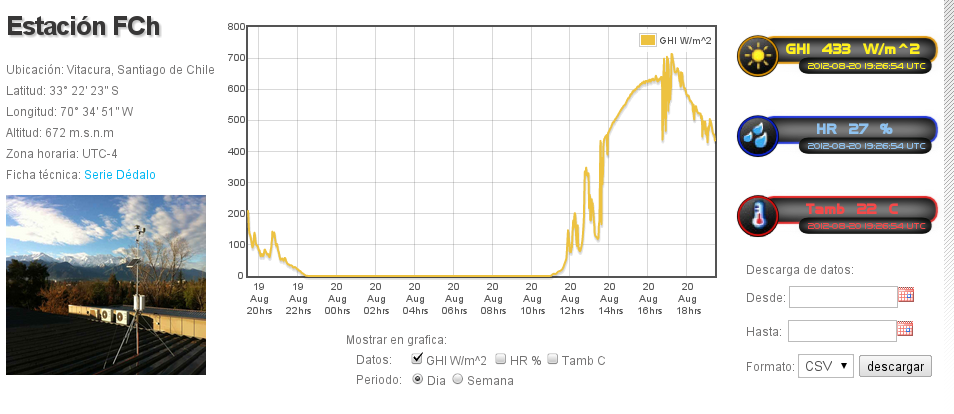
\includegraphics[scale=]{./images/cap5chap1img0}
	\caption{Presentacion de la aplicacion}
	\label{fig:figure1}
\end{figure}
A la izquierda en la primera columna la aplicacion muestra la informacion general de la estacion, presentando datos tales como su nombre, ubicacion politica y geografica, altitud, zona horaria donde se encuentra y finalmente una ficha tecnica sobre el hardware que posee. En la parte inferior se puede apreciar una fotografia de esta.

\begin{figure}[h]
	\begin{minipage}[b]{0.45\linewidth}
		\centering
		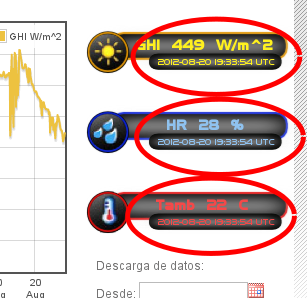
\includegraphics[width=\textwidth]{./images/cap5chap1img5-1}
		\caption{Primera marca}
		\label{fig:figure1}
	\end{minipage}
	\begin{minipage}[b]{0.45\linewidth}
		\centering
                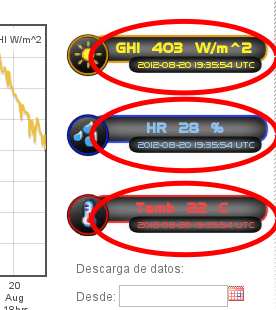
\includegraphics[width=\textwidth]{./images/cap5chap1img5-2}
                \caption{Segunda marca}
                \label{fig:figure1}
	\end{minipage}
\end{figure}
En la columna derecha de la aplicacion se presentan indicadores de la ultima medicion obtenida, por cada parametro que la estacion mide hay un ''widget'', esto, muestar el valor numerico de la medicion junto a sus unidades y nombre. En la zona inferirior de cada medicion se muestra la fecha a la que se asocia dicha medicion.

\subsubsection{Manejo del vizualizador}
\begin{figure}[ht]
        \centering
        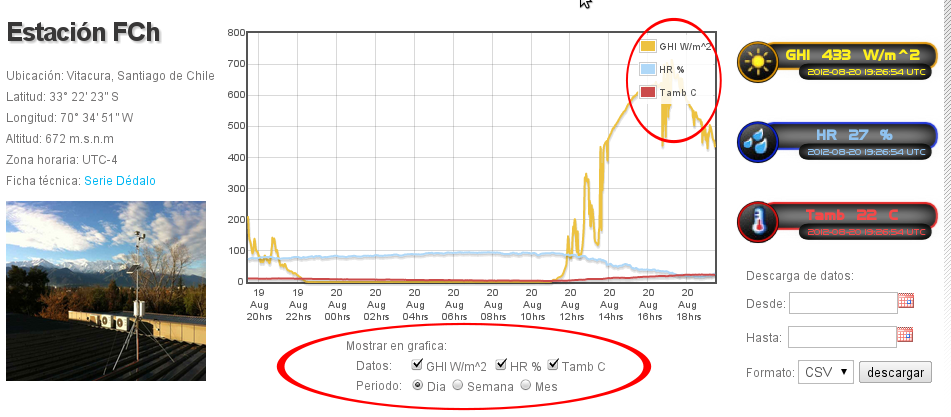
\includegraphics[width=\textwidth]{./images/cap5chap1img1}
        \caption{default}
        \label{fig:figure1}
\end{figure}
La primera herramienta de la cual dispone ''solarGraficos'' da la posibilidad de habilitar o desabilitar en la grafica las curvas para los diferentes parametros medidos por la estacion, estas pueden mostrarse de manere incividual o bien todas juntas.

\begin{figure}[ht]
        \centering
        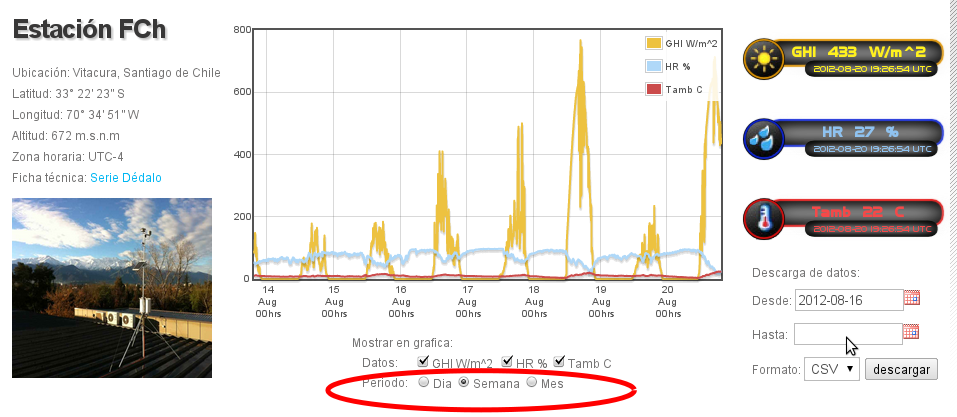
\includegraphics[width=\textwidth]{./images/cap5chap1img3}
        \caption{default}
        \label{fig:figure1}
\end{figure}
Siguiendo con las herramientas de configuracion de la grafica, la imagen \ref{fig} nos muestra la posibilidad de modificar los peridos de tiempo que se muestran para cada una de las diferentes curvas, dado que la cantiadad de datos con la que se dibujan las graficas son bastante grandes, estas toma algun tiempo en cargarse, por lo que si obsevamos con mas detalle, las opciones para mostrar las curbas en periodos de una semana, un mes o un año, iran apareciendo a medida que los datos esten totalmente cargados. Esta carga ocurren de manera trasparente por lo que mientras esto sucede el usuario puede hacer uso de todas las demas funcionalidades de la aplicacion.

\begin{figure}[ht]
	\begin{minipage}[b]{0.45\linewidth}
        	\centering
        	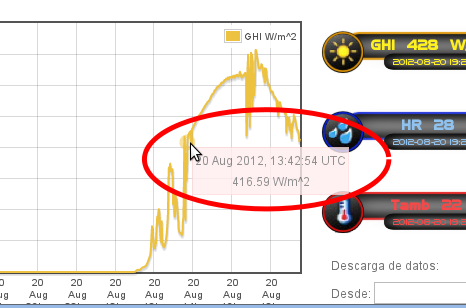
\includegraphics[width=\textwidth]{./images/cap5chap1img4-1}
        	\caption{default}
        	\label{fig:figure1}
	\end{minipage}
	\begin{minipage}[b]{0.45\linewidth}
                \centering
                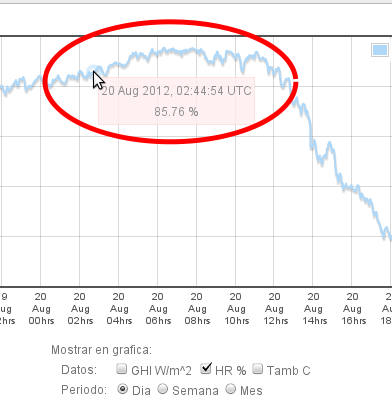
\includegraphics[width=\textwidth]{./images/cap5chap1img4-2}
                \caption{default}
                \label{fig:figure1}
        \end{minipage}
	\begin{minipage}[b]{0.45\linewidth}
                \centering
                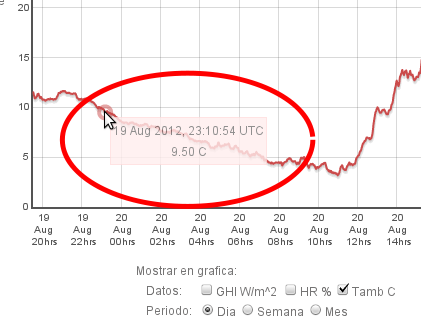
\includegraphics[width=\textwidth]{./images/cap5chap1img4-3}
                \caption{default}
                \label{fig:figure1}
        \end{minipage}
\end{figure}
Para obtener mas detalles respecto de alguna medicion en particular reflejada en la grafica, basta con posicionar el cursor sobre la curva deseada y esta identificara de manera automatica los puntos donde exista una medicion, identificando el punto con un circulo a su alrededor, adicionalmente mostrara una pequeña ventana emergente con informacion detallada de la medicion, udidades, hora y fecha especifica. Las imagenes \ref{fig} muestran como esta caracteristica se aplica a cada una de las curvas en conjunto como por separado.

\subsubsection{Descarga de datos}
\begin{figure}[ht]
	\begin{minipage}[b]{0.45\linewidth}
        	\centering
        	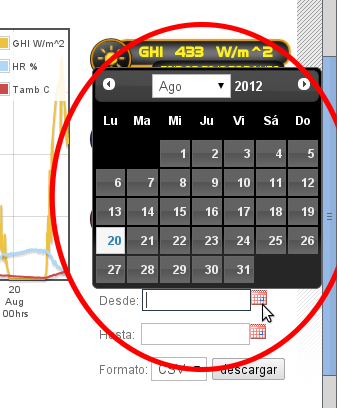
\includegraphics[width=\textwidth]{./images/cap5chap1img2-1}
        	\caption{default}
        	\label{fig:figure1}
	\end{minipage}
	\begin{minipage}[b]{0.45\linewidth}
	 	\centering
        	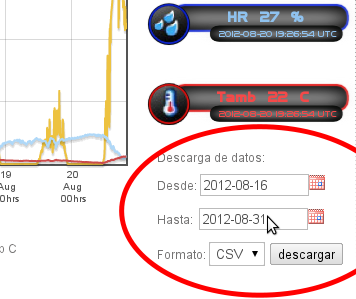
\includegraphics[width=\textwidth]{./images/cap5chap1img2-2}
        	\caption{default}
        	\label{fig:figure1}
	\end{minipage}
	\begin{minipage}[b]{0.45\linewidth}
		\centering
        	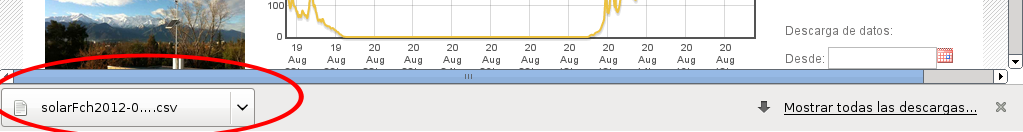
\includegraphics[width=\textwidth]{./images/cap5chap1img2-3}
        	\caption{default}
        	\label{fig:figure1}
	\end{minipage}
\end{figure}
La aplicacion cuenta con un modulo que permite descargar los datos directamente desde el ''Servidor de almacenamiento de datos'' de manera personalizada, para ellos en la seccion inferior derecha bajo el titulo ''Descarga de datos'' hay dos campos denominados ''desde'' y ''hasta'', al hacer click en cada uno de ellos se despliega un calendario que nos permite seleccionar el dia especifico para cada campo\ref{fig}. Mediante esta utilidad podemos especificar el rango de tiempo que contendra el fichero descargado con los datos en formto CSV \ref{fig}. Este fichero puede ser utilizado en diversas aplicaciones externeas para cargar los datos y realizar cualquier tipo de procesamiento deseado.

\clearpage 
\subsection{SolarCalc}
\subsubsection{Ingreso al sistema}
\begin{figure}[ht]
        \centering
        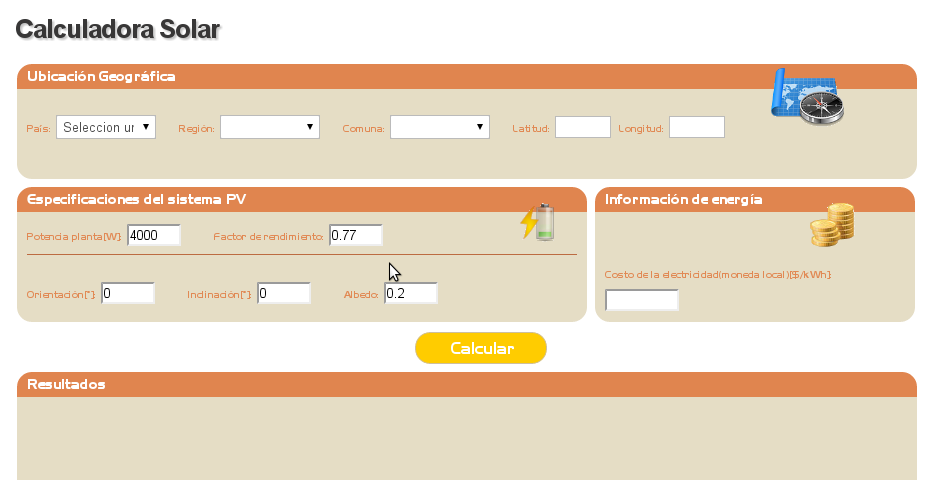
\includegraphics[width=\textwidth]{./images/cap5chap1img6}
        \caption{default}
        \label{fig:figure1}
\end{figure}
Al cargar la calculadora se aprecia la siguiguiente imagen \ref{fig}, adaptada a los requerimientos planteados, es una interfaz sencilla, con la menor cantidad de parametros necesarios, los cuales se van actualizando en tiempo real a medida que el usuario los rellena. Dividida en 4 secciones de acuerdo a la caracterizacion de los parametros requeridos.

\subsubsection{Ubicacion geografica}
La primera seccion que se debe rellenar es la posicion geografica donde se pretende instalar la planta a simular, por el momento la calculadora solo cuenta con informacion de Chile en todas sus Regiones y Comunas, al momento de seleccionar la comuna 
el sistema automaticamente establece las coordenas geograficas del centro de esta a modo referencial. Como indica la figura \ref{fig} los parametros deben ser ingresados en orden secuencial, iniciando por el pais, luego la region y finalmente la comuna, de manera de permitir al sistema ir cargando la informacion de fomra dinamica.
\begin{figure}[ht]
        \begin{minipage}[b]{0.45\linewidth}
                \centering
                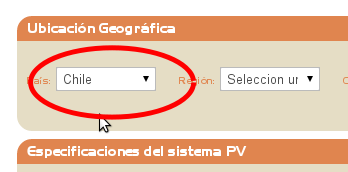
\includegraphics[width=\textwidth]{./images/cap5chap1img7-1}
                \caption{default}
                \label{fig:figure1}
        \end{minipage}
        \begin{minipage}[b]{0.45\linewidth}
                \centering
                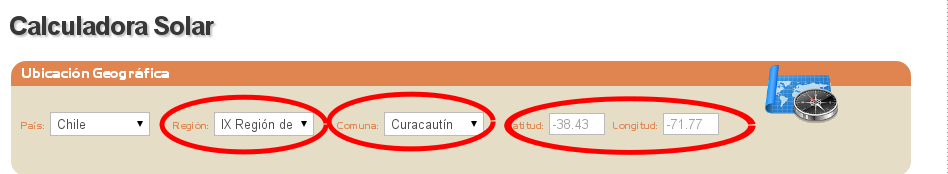
\includegraphics[width=\textwidth]{./images/cap5chap1img7-2}
                \caption{default}
                \label{fig:figure1}
        \end{minipage}
\end{figure}

\subsubsection{Especificaciones del sistema PV e informacion de la energia}
Esta seccion es una de las mas complejas si no se cuenta con cierto conocimiento tecnico de los sistemas fotovoltaicos, aca se debe proporcionar a la calculadora paramentros especificos (Ver Fig:\ref{fig}) de la configuracion de los equipos que quiere instalar en la planta a simular. Los parametros que deben ser ingresados se detallan a continuacion:\\
\begin{itemize}
\item[Potencia de la planta]
\item[Factor de rendimiento]
\item[Orientacion]
\item[Inclinacion]
\item[Albedo]
\item[Costo de la energia]
\end{itemize}

\begin{figure}[ht]
        \centering
        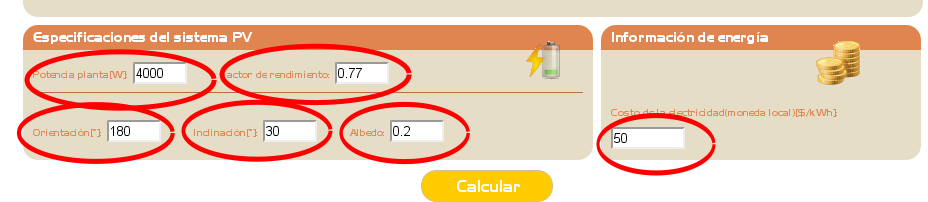
\includegraphics[width=\textwidth]{./images/cap5chap1img8}
        \caption{default}
        \label{fig:figure1}
\end{figure}

\subsubsection{Resultados}
Finalmente, luego de llenar toda la informacion solicitada, se debe hacer click en el boton ''calcular'', pasados unso segundos el sistema entregara un resultado dividio en 3 seccion principales (Ver Fig:\ref{fig}). La primera seccion es una tabla de resultados la cual nos informa mes a mes para un año tipico, la cantidad de radicion media, la cantidad de energia producida especificamente para los parametros de configuracion ingresados y el costo de venta que debiese tener la enrgia producida, este ultimo paramentro representa una utilidad en cuanto si se desea utilizar estos calculos en alguna propuesta economica para la instalacion de alguna planta.\\ La seguna seccion nos muestra en la parte inferior izquierda un grafico anual en el tiempo y dos ejes laterales, este grafico nos informa respecto de la eficiencia que tendra el sistema PV comparando la curba de radiacion con la curba de energia producida.\\ Finalmente el grafico de la para inferior derecha tiene como objetivo caracterizar la radicion solar en un año meteorologico tipico para cada mes del año con la cual se realizaron los calculos.
\begin{figure}[ht]
        \centering
        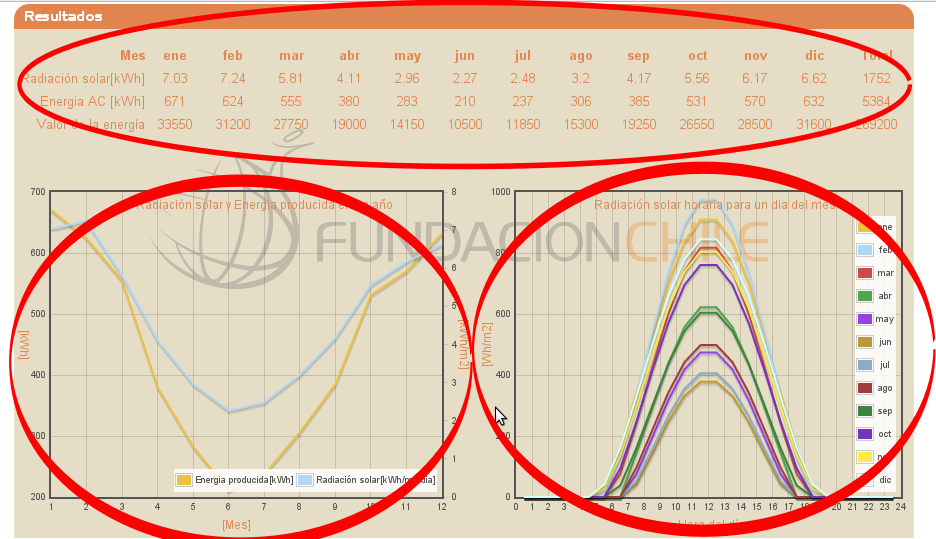
\includegraphics[width=\textwidth]{./images/cap5chap1img9}
        \caption{default}
        \label{fig:figure1}
\end{figure}

\section{Pruebas de comunicación}
Uno de los problemas más complejos que se enfrentó durante el desarrollo de esta Memoria fue el diseño e implementación de los sistemas de comunicación que permitieron establecer conexiones confiables y seguras entre las distintas componentes del sistema. De acuerdo al diseño planteado en el capítulo \ref{solucion}, se puede apreciar que la comunicación entre la componente de ''Aplicaciones'' y la de ''Almacenamiento de datos'' fue más o menos trivial dentro de lo que se refiere a la comunicación Web en un sistema informático, sin embargo, al momento de interconectar las ''Estaciones de medición'' con el resto del sistema hubo que considerar muchas variables extras tales como: geográficas, ambientales y eléctricas.

Las estaciones al estar ubicadas en lugares geográficos remotos en la mayoría de los casos no disponen de cables o conexiones a la red de datos. La señal de telefonía celular con buen soporte de datos no es de buena calidad en todos los lugares del país y con menor razón en lugares como el Desierto de Atacama (donde se ubica la planta), en medio de cordones montañosos e incluso en lugares más aislados. Las estaciones según requerimientos debían disponer de un sistema de comunicación flexible que pudiese ser adaptado a todas las condiciones y dificultades anteriormente mencionadas, para esto se diseño un sistema flexible, de forma que permite adaptar diferentes tecnologías de manera rápida y sencilla, sin embargo, para efectos prácticos de esta Memoria se implementaron dos módulos diferentes: Comunicación a través de Ethernet y comunicación vía módem de telefonía celular.

\subsection{Caso de Pruebas}
En las proximas secciones de este capitulo de exponene diferentes pruebas realizadas al sistema, entre ellas, la conectividad con las estaciones de medicion y los servidores de datos y aplicaciones, ademas se realizaron pruebas para verificar los metodos de calculo, la programacion y la correctitud de los resultados teoricos en comparacion con resultados empiricos. Para las pruebas de comunicacion se utilizo una estacion Dedalo (\ref{anexo}), denomidada en capitulos anteriores como ''Estacion Fch'' la cual es la estacion ubicada en las dependecias de Fundacion Chile en la comuna de Vitacura de la Region Metropolitana, esta estacion durante el periodo de prueba midio: Radicion solar global en el plano horizontal, Temperatura ambiente y humedad relativa del aire. Ademas se considera el periodo de prueba como el funcionamiento normal entre las fechas de Mayo del 2012 y Septiembre 2012, considerando de forma especial una interrupcion programada en el mes de Agosto para mantencion de los instrumentos por el periodo de una semana y 6 interrupciones no programadas por fallos en la conectividad del sistemas inferiores a 6 horas de funcionamiento cada una durante todo el periodo producto del funcionamiento defectuso de una bateria de la estacion lo cual dejo a esta sin electricidad en dichas ventanas de tiempo, una vez diagnosticado el problema se procedio a reemplazar la bateria defectuosa solucionando asi el problema.\\
Para la comparacion teorica de los calculos se utilizaron bases de datos elaboradas por xxxx considerando muestras de un año meteorologico tipico(referencia o pie de pagina) para la comunas de Vitacura, Antofagasta y Concepcion.  
 
\subsection{Comunicación de estación ''VitacuraFCh'' con ''Servidor de datos'' - Vía Ethernet}
Una de los primeras actividades que se realizó en esta Memoria fue la interiorización con los equipos que componen las estaciones meteorológicas, esto involucró el aprender a utilizar elementos de hardware tales como el ''datalogger'' Campbell Scientific CR1000, módems de telefonía celular y otras interfaces de comunicación.\\
Para lograr que la estación se comunique de forma autónoma con el ''Servidor de almacenamiento de datos'' fue necesario escribir un programa para el ''datalogger'' que fuese capaz de realizar una petición GET a través del módulo ''Campbell NL200'' utilizando la implementación del protocolo TCP/IP de esta Interfaz.
Para esto fue necesario conectar el módulo ''NL200'' a través de la interfaz ''SCI/O'' del ''datalogger'' y configurar el módulo para actuar en modo ''bridge'', esto permite una Comunicación transparente entre el ''datalogger'' y la red informática de Fundación Chile.

Esta modalidad del sistema de comunicación es bastante limitada, ya que es necesario contar en los lugares de instalación de las estaciones con una infraestructura de red de datos informática, ya que a la estación se le debe proporcionar un punto de red vía cable de red.

Para verificar el estado de la conexión se exponen dos métodos, en primer lugar la conexión manual utilizando el software proporcionado por el fabricante ''PC400'', a través de este software establecemos una conexión ''TCP/IP'' utilizando la dirección IP asignada a la estación y realizamos una prueba de descarga de datos:

\begin{enumerate}
\item Ejecutar el PC400
\item Creamos una nueva conexión(Ver Fig:\ref{pruebas1}) 
\item En la sección ''comunicación setup'', seleccionamos el dispositivo ''CR1000'' y luego seleccionamos el tipo de convección ''Ip Port''.
\item Ingresamos la dirección IP de la estación y finalizamos la configuración(Ver Fig:\ref{pruebas2}).
\item En la pantalla principal, en el menú de la izquierda seleccionamos la nueva interfaz y presionamos el botón ''connect''(Ver Fig:\ref{pruebas3})
\item Una vez establecida la conexión vamos a la solapa superior que dice ''monitor data'' y podemos observar los parámetros que la estación esta midiendo(Ver Fig:\ref{pruebas4}).
\item Finalmente vamos a la solapa ''collect data'', presionamos en ''collect'' y esperamos a que se complete la descarga(Ver Fig:\ref{pruebas5}).
\end{enumerate}

\begin{figure}[h!]
        \centering
        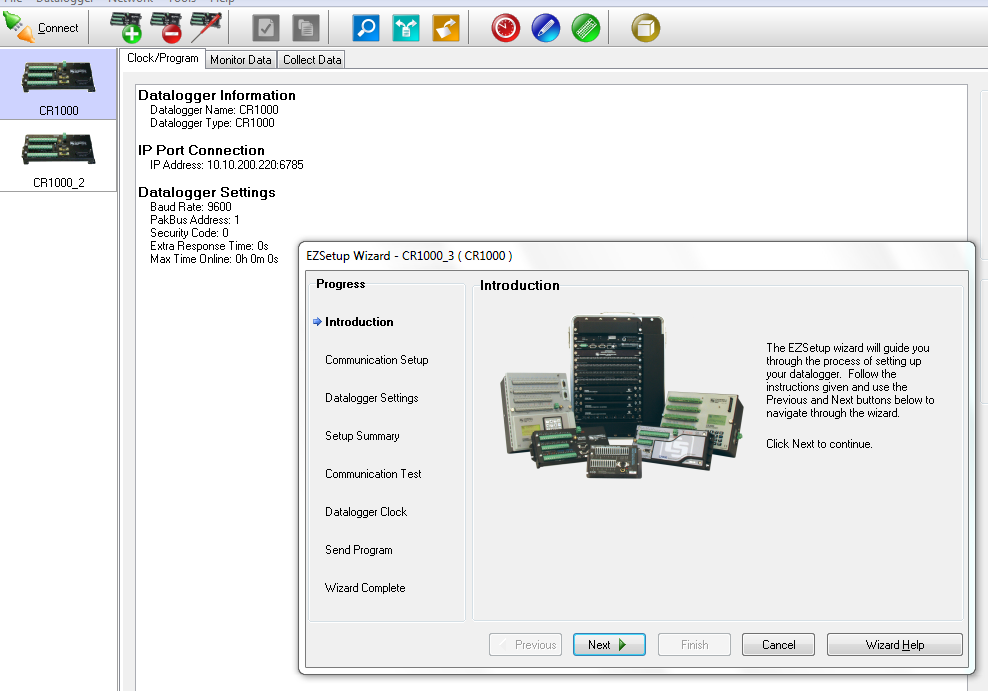
\includegraphics[width=300pt]{images/pruebas1}
        \caption{Crear nueva conexión}
        \label{pruebas1}
\end{figure}
\begin{figure}[h!]
        \centering
        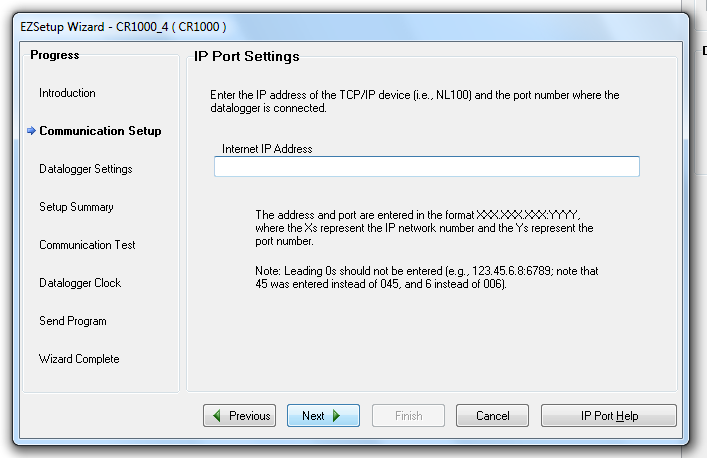
\includegraphics[width=300pt]{images/pruebas2}
        \caption{Ingresar dirección IP}
        \label{pruebas2}
\end{figure}
\begin{figure}[h!]
        \centering
        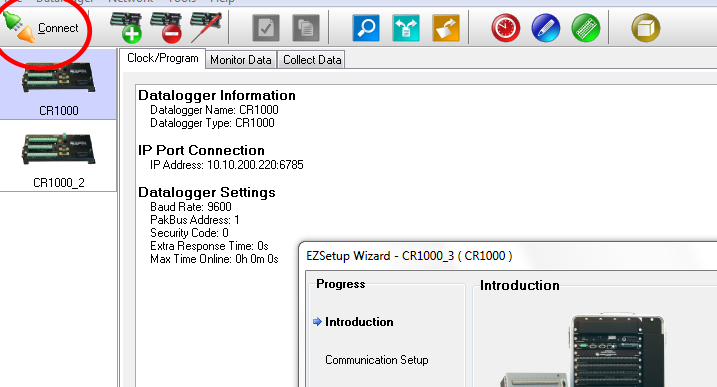
\includegraphics[width=300pt]{images/pruebas3}
        \caption{Estableciendo conexión}
        \label{pruebas3}
\end{figure}
\begin{figure}[h!]
        \centering
        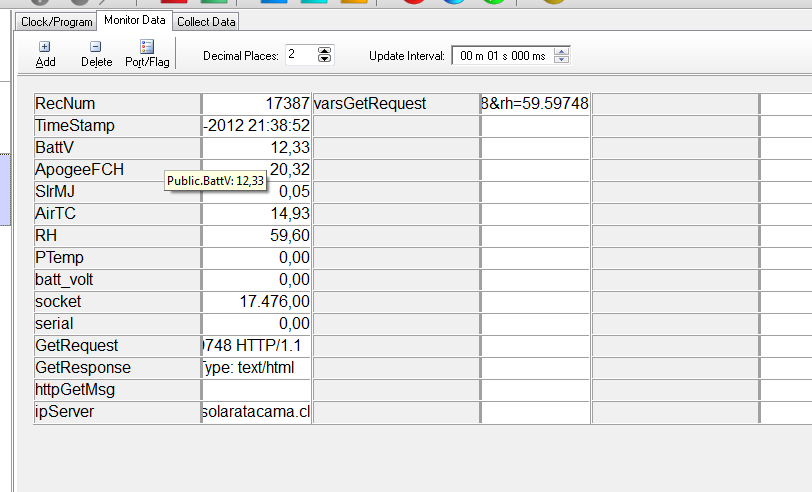
\includegraphics[width=300pt]{images/pruebas4}
        \caption{Monitores datos de estación}
        \label{pruebas4}
\end{figure}
\begin{figure}[h!]
        \centering
        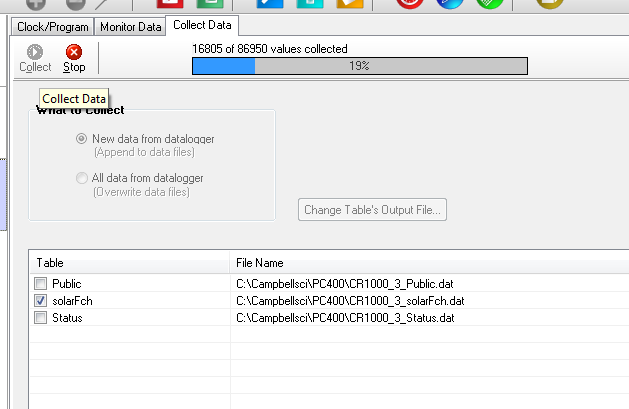
\includegraphics[width=300pt]{images/pruebas5}
        \caption{Descarga de datos}
        \label{pruebas5}
\end{figure}

\subsection{Comunicacion de las estacion ''VitacuraFch'' con el ''Servidor de datos''}
Para verificar la conexión autónoma desde la estación hacia la red de datos mediante la programación del datalogger(Ver Fig:\ref{pruebasLog1}). En el se puede a preciar el registro del servidor Web Apache HTTPD cuando la estación realiza la petición GET.

\begin{figure}[h!]
        \centering
        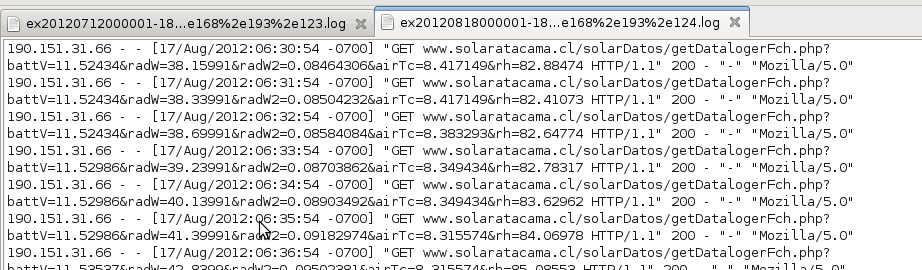
\includegraphics[width=300pt]{images/pruebasLog1}
        \caption{Logs Apache HTTPD - Comunicación con estación meteorológica}
        \label{prubasLog1}
\end{figure}m

\subsection{Comunicación de estación ''VitacuraFCh'' con ''Servidor de datos'' - Vía Módem telefonía celular}
Este tipo de comunicación es el segundo método que se implementó en esta memoria y en comparación al método anterior es mucho mas flexible ya que es posible establecer comunicación con estaciones de forma inalámbrica en diferentes ubicaciones de la geografía nacional, incluso en lugares remotos donde es posible recibir señal de la red telefonía celular. Actualmente el desarrollo de esta tecnología en nuestro país, permite establecer comunicación en lugares bastante remotos como sectores montañosos en la cordillera o bien en medio del Desierto de Atacama.

Para testear la comunicación mediante este modulo de utiliza el software proporcionado por el fabricante del ''datalogger'', el ''PC400'' siguiendo los siguientes pasos:

\begin{enumerate}
\item Ejecutar el PC400n
\item Creamos una nueva conexión(Ver Fig:\ref{pruebas1})
\item En la sección ''comunicación setup'', seleccionamos el dispositivo ''CR800'' y luego seleccionamos el tipo de convección ''Phone Modem'' y luego la opcion ''Use modem from CSI list''.
\item Seleccionamos el puerto COM donde esta conectado el modem y en la lista siguiente selecionamos el modelo del moden que vamos a utilizar, Para este caso particular fue necesario configurar un nuevo modem).
\subitem Para configurar un nuevo modem, hacemos click en ''Edit Modem Database'', luego bajo la lista que hay en la nueva ventana desplegada hacemos click en ''New'', ingresamos el nombre del nuevo modem y presionamos ''OK''
\subitem Finalmente editamos los parametros del nuevo modem. ''Rset strng'' lo seteamos en blanco y ''Initialization Strin'' lo dejamos en \textbf{\&C0\&D0}, luego hacemos click en ''Save''. 
\item Una vez configurado el modem ingresamos el ''Phone Number'', numero de telefono que tienen el modem al cual vamos a llmar y presionamos en ''Next'' para ir al siguiente paso.
\item En esta nueva ventana configuramos el ''Baud Rate'' en \textbf{9600} y Finalizamos la configuracion.
\item Finalmente hacemos click en el boton superior izquierdo con la nueva conexion seleccionada para arir un canal de comunicacion con la estacion.
\item Una vez establecida la conexión vamos a la solapa superior que dice ''monitor data'' y podemos observar los parámetros que la estación esta midiendo(Ver Fig:\ref{pruebas4}).
\item Finalmente vamos a la solapa ''collect data'', presionamos en ''collect'' y esperamos a que se complete la descarga(Ver Fig:\ref{pruebas5}).
\end{enumerate}
\begin{figure}[h!]
        \centering
        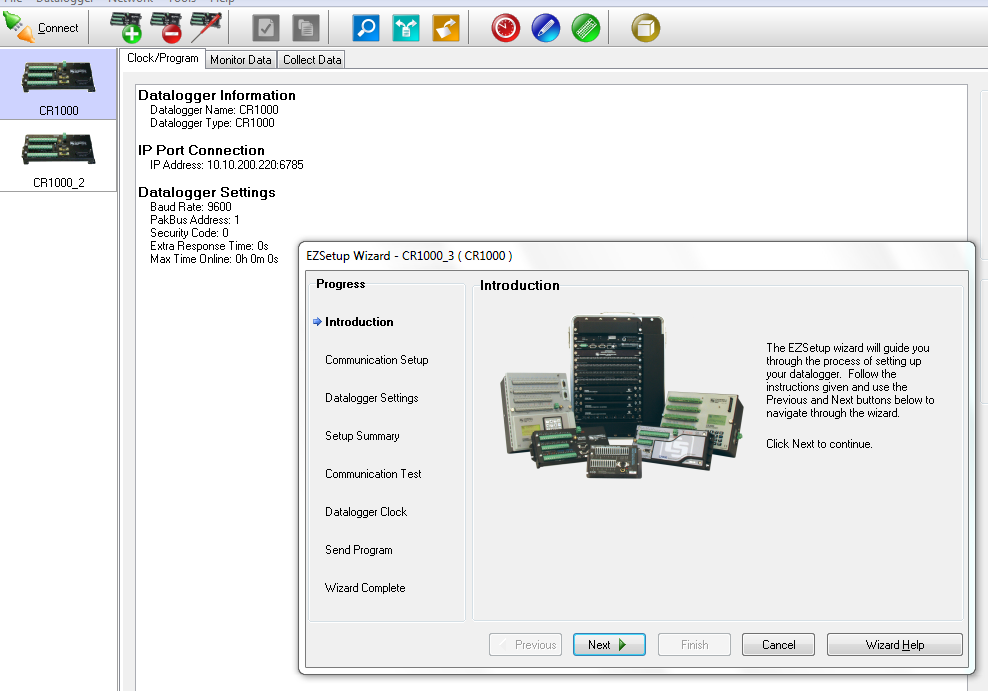
\includegraphics[width=300pt]{images/pruebas1}
        \caption{Crear nueva conexión}
        \label{pruebas1}
\end{figure}
\begin{figure}[h!]
        \centering
        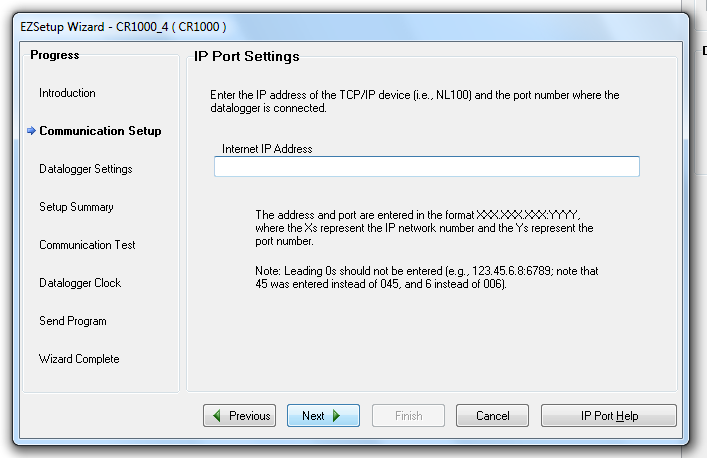
\includegraphics[width=300pt]{images/pruebas2}
        \caption{Ingresar dirección IP}
        \label{pruebas2}
\end{figure}
\begin{figure}[h!]
        \centering
        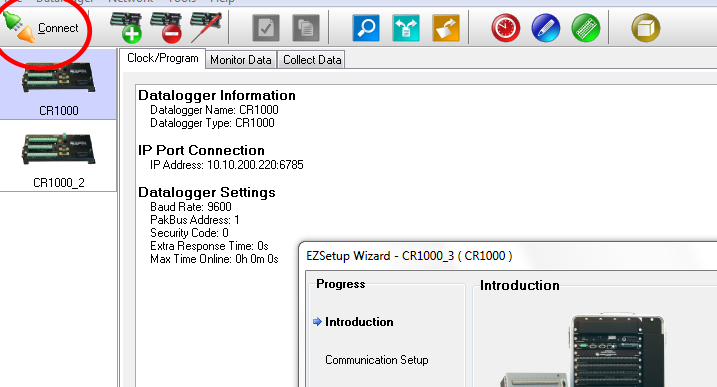
\includegraphics[width=300pt]{images/pruebas3}
        \caption{Estableciendo conexión}
        \label{pruebas3}
\end{figure}
\begin{figure}[h!]
        \centering
        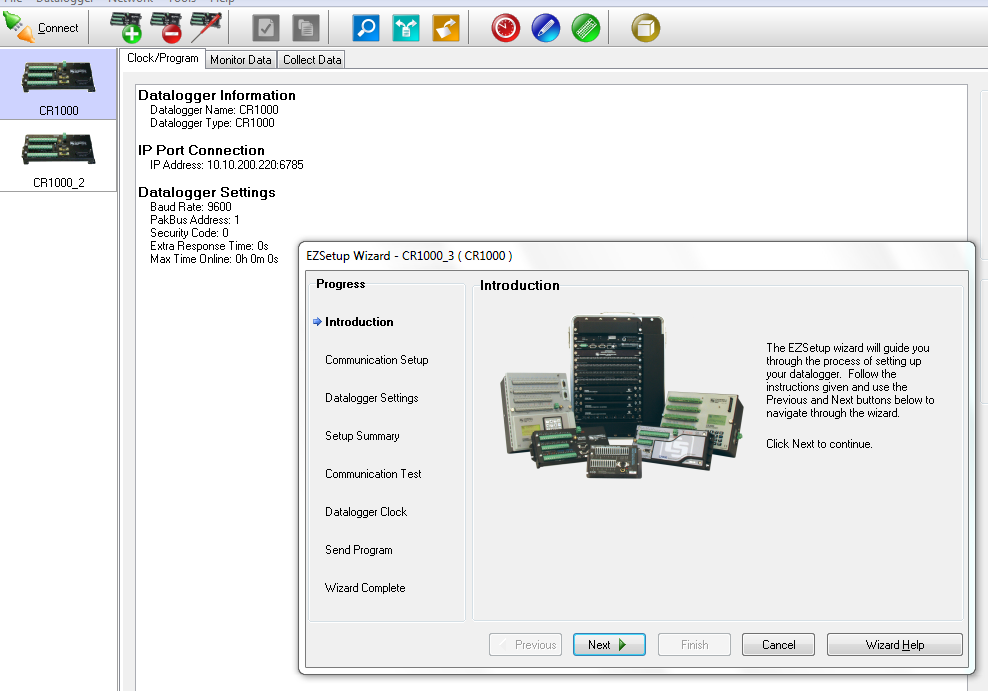
\includegraphics[width=300pt]{images/pruebas1}
        \caption{Crear nueva conexión}
        \label{pruebas1}
\end{figure}
\begin{figure}[h!]
        \centering
        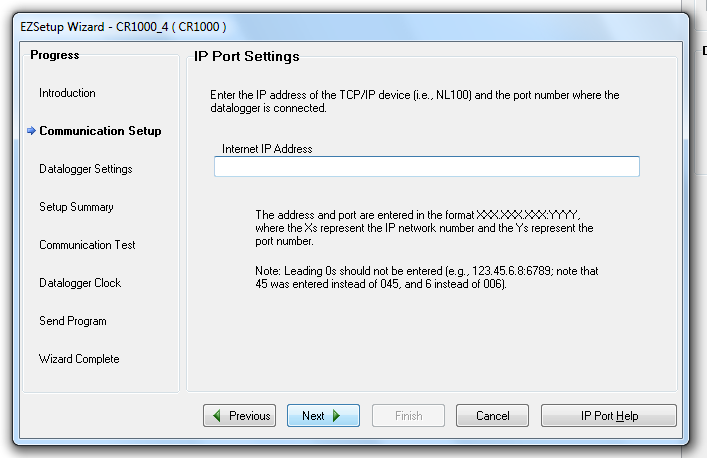
\includegraphics[width=300pt]{images/pruebas2}
        \caption{Ingresar dirección IP}
        \label{pruebas2}
\end{figure}
\begin{figure}[h!]
        \centering
        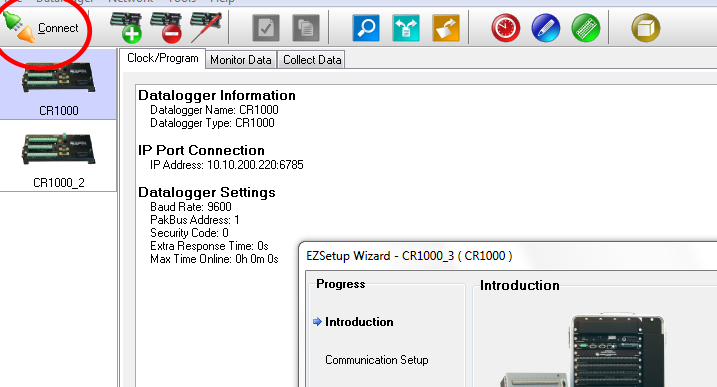
\includegraphics[width=300pt]{images/pruebas3}
        \caption{Estableciendo conexión}
        \label{pruebas3}
\end{figure}

\section{Verificación de datos}
Una ves desarrollado el sistema con todas las aplicaciones que cubren los requerimientos planteados en la sección inicial(\ref{alcances}) de esta memoria es necesario verificar que los datos obtenidos sean correctos y de la misma forma los cálculos a los que estos son sometidos.\\
Ha quedado expresado en la sección de requerimientos que la confiabilidad de los datos así como del proceso de calculo es esencial en el funcionamiento del sistema, pequeños errores en el sistema de calculo podrían significar grandes errores en el dimensionamiento de los sistemas fotovoltaicos, lo que podría traer con secuencia poco deseables a los actores de la RedSolLAC.\\
Es necesario recordar que durante el desarrollo de esta Memoria se creo un nuevo método de calculo que intenta mejorar sistemas anteriores por lo que es sumamente necesario comprobar y exponer las diferencias en los resultados obtenidos, así como de resaltar las mejoras que este nuevo método propone.\\

Los resultados obtenidos fueron comparados con diferentes fuentes de datos así como con diferentes modelos de cálculos, algunos de ellos, los mas relevantes, son presentados a continuación junto con el análisis correspondiente a las diferencias encontradas.\\
La primera verificacion apunta a comprovar que el modelo matematico haya sido bien implementado, luego se presentan 3 resultados obtenidos con la calculadora desarrollada y 2 sistemas externos, finalmente comparamos los resultados teoricos con los obtenidos en un sistema PV en operacion.\\

\subsection{PVWatts}
A la fecha de desarrollo de esta Memoria es el único software en formato Web existente que ofrece el servicio de calculo y dimensionamiento de sistemas fotovoltaicos que cuenta con información para algunas localidades en Latinoamérica. Sin embargo en su método de calculo implementa un modelo basado en la ''media de la radiación mensual''.\\ 
\subsection{PVSyst}
Es un software privativo, de uso profesional para el sector de la industria energética solar. Este software permite diseñar, estudiar, dimensionar y simular sistemas fotovoltaicos, con un método de calculo bastante complejo y cercano al funcionamiento real de una planta solar fotovoltaica considerando complejas variables que influyen en el calculo, tales como el sombreado producido por los mimos módulos del sistema o la sombra generada por cerros cercanos a las instalaciones.\\

\subsection{Comparación ''solarCalc'' con ''Plataforma Web para sistemas térmicos''}
La ''Plataforma Web para sistemas térmicos'' se presenta como el trabajo de Memoria de fin de titulo de magíster del ingeniero correferente de esta Memoria\cite{memoriaEdo}. Este trabajo es una de las bases con las cuales se diseño el sistema de calculo implementado en la calculadora. Para el proceso de verificación se utiliza una ''macro en excel'' originada en dicho trabajo de titulo y los resultados entregados en modo de depuracion por la calculadora.\\
mediante este método se pretende verificar que la implementación de la calculadora sea correcta y entregue los valores esperados.

\begin{table}[h!]
\caption{Resultados verificacion de ecuaciones macro excel}
\begin{tabular}{|l|c|c|c|c|c|c|c|c|}
        \hline
        \textbf{Resultados macro exel}&&&&&&&&\\
        \hline
        \textbf{Hora del dia}&0.5&1.5&2.5&3.5&4.5&5.5&6.5&7.5\\
        \hline
        \textbf{Radiacion Global Horizontal horaria}&0&0&0&0&0&20.6&203.3&421.1\\
        \hline
        \textbf{Radiacion Difusa Horizontal horaria}&0&0&0&0&0&5.9&51.5&95.6\\
        \hline
        \textbf{Radiacion Directa Horizontal horaria}&0&0&0&0&0&14.7&151.8&325.5\\
        \hline
\end{tabular}
\begin{tabular}{|c|c|c|c|c|c|c|c|}
        \hline
        &&&&&&&\\
        \hline
        8.5&9.5&10.5&11.5&12.5&13.5&14.5&15.5\\
        \hline
        650.8&862.4&1025.2&1113.7&1113.7&1025.2&862.4&650.8\\
        \hline
        135.1&167.4&190.2&202&202&190.2&167.4&135.1\\
        \hline
        515.7&695.1&835&911.7&911.7&835&695.1&515.7\\
        \hline
\end{tabular}
\begin{tabular}{|l|c|c|c|c|c|c|c|c|c|}
        \hline
        \textbf{Resultados macro exel}&&&&&&&&&\\
        \hline
        \textbf{Hora del dia}&16.5&17.5&18.5&19.5&20.5&21.5&22.5&23.5&Total\\
        \hline
        \textbf{Radiacion Global Horizontal horaria}&421.1&203.3&20.6&0&0&0&0&0&8594.2\\
        \hline
        \textbf{Radiacion Difusa Horizontal horaria}&95.6&51.5&5.9&0&0&0&0&0&1695.4\\
        \hline
        \textbf{Radiacion Directa Horizontal horaria}&325.5&151.8&14.7&0&0&0&0&0&6899\\
        \hline
\end{tabular}
\end{table}

\begin{table}[h!]
\caption{Resultados verificacion de ecuaciones calculadora}
\begin{tabular}{|l|c|c|c|c|c|c|c|c|c|c|c|c|c|c|c|c|c|c|c|c|c|c|c|c|c|}
        \hline
        \textbf{Resultados calculadora}&&&&&&&&&&&&&&&&&&&&&&\\
        \hline
        \textbf{Hora del dia}&0.5&1.5&2.5&3.5&4.5&5.5&6.5&7.5&8.5&9.5&10.5&11.5&12.5&13.5&14.5&15.5&16.5&17.5&18.5&19.5&20.5&21.5&22.5&23.5&Total\\
        \hline
        \textbf{Radiacion Global Horizontal horaria}&0&0&0&0&0&21&204&421&651&862&1025&1114&1114&1025&862&651&421&204&21&0&0&0&0&0&8596\\
        \hline
        \textbf{Radiacion Difusa Horizontal horaria}&0&0&0&0&0&6&52&96&135&167&190&202&202&190&167&135&96&52&6&0&0&0&0&0&1696\\
        \hline
        \textbf{Radiacion Directa Horizontal horaria}&0&0&0&0&0&15&152&325&516&695&835&912&912&835&695&516&325&152&15&0&0&0&0&0&6900\\
        \hline
\end{tabular}
\end{table}

\subsection{''solarCalc'' v/s ''PVWatts'' v/s ''PVSist con datos de Antofagasta}
El objetivo de realizar esta comparación es exponer las diferencias que se generan por la utilización de los diferentes modelos de cálculo y verificar si las mejoras propuestas son significativas.

\begin{table}[h!]
\caption{Comparacion de software con datos de Antofagasta}
\begin{tabular}{|c|c|c|c|c|}
        \hline
	\textbf{Mes}&\textbf{Antofagasta (kWh/m2/dia)}&\textbf{Energia estimada PVWatts (kWh)}&\textbf{Energia estimada solarCalc (kWh)}&\textbf{Energia estimada PVSist (kWh)}\\
	Ene&	7.70&	630&	662&	652\\
        \hline
	Feb&	7.62&	593&	627&	622\\
        \hline
	Mar&	6.71&	642&	666&	686\\
        \hline
	Abr&	5.48&	570&	578&	617\\
        \hline
	May&	4.12&	472&	475&	527\\
        \hline
	Jun&	3.63&	423&	423&	471\\
        \hline
	Jul&	3.75&	444&	443&	492\\
        \hline
	Ago&	4.65&	514&	522&	569\\
        \hline
	Sep&	5.68&	556&	565&	595\\
        \hline
	Oct&	6.68&	620&	630&	645\\
        \hline
	Nov&	6.96&	578&	593&	579\\
        \hline
	Dic&	7.63&	620&	648&	636\\
        \hline
	Total&5.87&	6662&	6832&	7089\\
        \hline
\end{tabular}
\end{table}

\subsection{''solarCalc'' v/s ''PVWatts'' v/s ''PVSist con datos de Vitacura}
El objetivo de realizar esta comparación es verificar que tan cercano o confiable es el resultado obtenido por la calculadora y dimensionar la influencia de variables complejas.

\begin{table}[h!]
\caption{Comparacion de software con datos de Vitacura}
\begin{tabular}{|c|c|c|c|c|}
        \hline
	\textbf{Mes}&\textbf{Vitacura (kWh/m2/dia)}&\textbf{Energia estimada PVWatts (kWh)}&\textbf{Energia estimada solarCalc (kWh)}&\textbf{Energia estimada PVSist (kWh)}\\
	Ene&	7.6&	641&	649&	609\\
        \hline
	Feb&	7.45&	563&	628&	609\\
        \hline
	Mar&	6.39&	550&	678&	684\\
        \hline
	Abr&	4.69&	393&	556&	595\\
        \hline
	May&	3.29&	288&	452&	516\\
        \hline
	Jun&	2.75&	233&	395&	440\\
        \hline
	Jul&	2.77&	245&	390&	434\\
        \hline
	Ago&	3.81&	340&	483&	539\\
        \hline
	Sep&	4.74&	407&	505&	526\\
        \hline
	Oct&	5.6&	492&	541&	545\\
        \hline
	Nov&	7.11&	592&	606&	583\\
        \hline
	Dic&	7.09&	600&	598&	592\\
        \hline
	Total&	5.26&	5344&	6481&	6673\\
        \hline
\end{tabular}
\end{table}

\subsection{''solarCalc'' v/s ''PVWatts'' v/s ''PVSist con datos de Concepcion}

\begin{table}[h!]
\caption{Comparacion de software con datos de Concepcion}
\begin{tabular}{|c|c|c|c|c|}
        \hline
	\textbf{Mes}&\textbf{Concepcion (kWh/m2/dia)}&\textbf{Energia estimada PVWatts (kWh)}&\textbf{Energia estimada solarCalc (kWh)}&\textbf{Energia estimada PVSist (kWh)}\\
	Ene&	7.64&	662&	688&	628\\
        \hline
	Feb&	6.81&	574&	597&	603\\
        \hline
	Mar&	4.93&	511&	521&	639\\
        \hline
	Abr&	3.39&	381&	383&	575\\
        \hline
	May&	1.89&	218&	232&	375\\
        \hline
	Jun&	1.54&	180&	193&	327\\
        \hline
	Jul&	1.79&	220&	232&	405\\
        \hline
	Ago&	2.53&	292&	301&	460\\
        \hline
	Sep&	3.97&	422&	423&	557\\
        \hline
	Oct&	5.42&	530&	540&	593\\
        \hline
	Nov&	6.55&	568&	586&	557\\
        \hline
	Dic&	7.54&	641&	669&	597\\
        \hline
	Total&	4.49&	5198&	5365&	6315\\
        \hline
\end{tabular}
\end{table}

\subsection{Comparacion con sistema PV en operacion}
La ultima verificación a la cual se ha sometido la aplicación construida es una verificación empírica. Utilizando un sistema fotovoltaico en operación, se ha obtenido una muestra de un día de mediciones, luego esta muestra se ha comprado con la predicción de la calculadora. Si bien la muestra obtenida en un día de prueba es poco significativo en comparación a los datos de todo un año sabemos que el comportamiento solar es cíclico y su unidad más pequeña es un día, por lo que esta medición se puede comparar con el resultado de un mes en particular. Este resultado nos da una orientación respecto del máximo error cometido entre un sistema teórico de cálculo y un sistema solar fotovoltaico operativos.

(tabla de datos)

